\section{Algorithmic Methods}
\label{sec:algorithms}
Our authoring interface relies on audio transcription and text alignment algorithms to link the master-script to the audio recordings.  

\subsection{Transcribing the audio recording}
We use IBM Speech to Text Service \cite{ibmspeechtotext} to obtain a verbatim transcript of each audio recording in real-time. The service outputs a time stamp for each word indicating its start and end time within the audio. It also segments the transcript into \textit{utterances} where each utterance is separated by a longer silent gap in the speech (longer than 500 ms). While automatic speech recognition is imperfect, we have found that in most cases the results were accurate enough for the purpose of alignment (below) and for users to understand the transcript. 
  
\subsection{Aligning the transcript to the master-script}
To support our side-by-side \textit{compare-view} as well as the \textit{All} tab view, we must identify corresponding parts of the master-script and recording transcripts. Moreover, we must partition these corresponding parts into segments that users can easily compare and merge into the master-script. Ideally, our segments should respect natural boundaries such as punctuations and line breaks in written text to aid readability. As discussed earlier, the segment boundaries should also align with longer pauses in the audio so that merge operations do not introduce obvious audio artifacts. Finally, we also want to separate parts of the transcript that generally agree with the master-script (i.e., planned speech) from parts that do not (i.e., improvised speech).  We designed a scoring function that optimizes for these requirements and use an iterative algorithm to co-segment the two texts. We first explain the algorithm and then describe the scoring function in detail.
\begin{figure}
\centering
  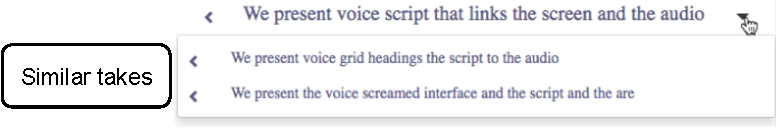
\includegraphics[width=1.0\columnwidth]{figures/multipletakes}
  \caption{The \textit{all-tab} groups alternative takes of a segment and dispalys them in a drop-down list. Users can click on each to compare the audio, and select one to \textit{accept} to the final track.  }~\label{fig:multipletakes}
\end{figure}

\textbf{Iterative co-segmentation}
Before running our co-segmentation algorithm, we first compute the global word-to-word alignment between each recording transcript and the master-script using the Needleman-Wunsch (NW) algorithm \cite{needleman1970general}. NW allows for insertions and deletions, which account for differences in the two texts, for example, due to rough scripts, inaccurate speech, or transcription errors.
%
The segmentation of the master-script depends on the segmentation of the transcript and vice versa. Our iterative algorithm alternates between optimally segmenting the master-script and the transcript independently using the result from one to segment the other. We initialize the segment boundaries at punctuations (.!?:;) in the unrecorded text and longer silent gaps ($>$\ 500ms)\ in the recorded text. In practice, we
found that two iterations were sufficient to converge to a solution.


For each optimization step, we use the classic optimal line-breaking algorithm by Knuth and Plass \cite{knuth1981breaking}: Given a text as a sequence of $n$ words $T = \{w_0,\dots,w_n\}$, the algorithm finds the optimal set of inter-word
boundaries that break the text into segments. We refer to the boundary between $w_i$ and $w_{i+1}$ as
$b_i$.
%
The algorithm iterates through each word, and for each $w_i$
computes and records the optimal set of text segments $S_i$ for words up to $b_i$, along with the total score $E(S_i)$ of
this partial solution. To determine the optimal partial solution for $w_i$, it
considers each previous boundary $b_j$ $(j<i)$, and evaluates two possible ways of
segmenting the text $T_{ji} = \{w_\text{j+1},
\dots,w_\text{i}\}$: 1) appending $T_{ji}$ to the last segment in $S_j$, or 2) forming a new text segment with $T_{ji}$. The algorithm selects the better (lower) of the two scores for $T_{ji}$ and adds it
to $E(S_j)$ to obtain the total score for the proposed
segmentation. After considering all candidate boundaries $b_j$, the partial solution with the minimum segmentation score is taken. Once the algorithm iterates through all the words, $S_n$ is the
optimal set of segments for the entire text. 

\textbf{Scoring function}
The dynamic programming algorithm described above requires a
scoring function ($E$) that evaluates the goodness of candidate text segments. We define this scoring function
based on three terms: 
\begin{enumerate}
\item{\textit{Punctuation and silent gaps}: We prefer segment boundaries after sentence punctuations, and in case of recorded text, where there is a longer silence gap. Placing cuts at silent gaps allows audio segments from different takes or different parts of a single take to be joined seamlessly. More precisely, we define the boundary score ($e_b$) for a single text segment $T_{ji} = \{w_\text{j+1}
\dots,w_\text{i}\}$ as:
\begin{equation}
    e_b(T_{ji})= 
\begin{cases}
   1.0, \text{ if } w_i \text{ is unrecorded w punctuation (.!?:;)}\\
   -1.0 \text{ if } w_i \text{ is unrecorded w/o punctuation}\\
   t_{gap}(w_{i}) \text{ if } w_i \text{ is recorded} 
\end{cases}
\end{equation}

where $t_{gap}(w)$ is the silence gap in seconds after a recorded word, $w$, and is equal to 1.0 for $w$ that is at the end of a recording.
\VREV{Note that it is important to consider both the sentence punctuations and the silent gaps. As the examples in} \VTODO{Figure~\ref{fig:scoring_example}} \VREV{illustrate, considering only puncutations can result in audio artifacts when merging recordings, and similarly, considering only utterance boundaries can produce unnatural cuts in the middle of a scripted sentence.}
}

\item{\textit{Global alignment}: We try to separate transcript segments that have a counterpart in the master-script from those that do not (planned vs. improvised), and vice versa (recorded vs. unrecorded). We utilize the global alignment output from the Needleman-Wunsch (NW) algorithm. For each word $w_i$ in one text ($T$) NW outputs a mapping ($M_{TT'}$) 
to the other text ($T'$), and vice versa. For instance, $M_{TT'} = \{m_0, \dots,m_n\}$ where $m_i$ is the index of the word in  $T'$ that matches $w_i$. $m_i < 0$ if the word has no match. We prefer text segments that have the proportion of matching words close to 0 or 1. The alignment score ($e_a$) for a single text segment $T_{ji}$ is:  
\begin{equation}
e_{a}(T_{ji}) = 2\times\bigg|\sum_{n=j+1}^{i}{match(w_n)}\big/(i-j) - 1/2 \bigg|
\end{equation}
where $match(w_i)$ is 1 or 0, depending on whether $m_i \geq 0$ or not (whether the word has a match or not).
}
\item{\textit{Consistency with the other text}: Since the end goal is to align the segments from both texts, we would like the segment boundaries from one text to align with the segment boundaries in the other text \VREV{even when the punctuation and utterance boundaries do not coincide}. Let $S' = \{s'_0, \dots, s'_n\}$ be the segmentation of text $T'$, where $s'_i$ is the index of the segment that word $w'_i$ belongs to. Given this segmentation and the mapping of $T$ to $T'$ from NW  ($M_{TT'}$), the consistency score ($e_c$) for a text segment $T_{ji}$ is:
\begin{equation}
    e_c(T_{ji})= 
\begin{cases}
   1.0, \text{ if } s'_{m_i} \neq s'_{m_k} \text{ for the smallest } k>i, m_k \geq0\\
   -1.0 \text{ otherwise }
\end{cases}
\end{equation}

$s'_{m_i}$ is the index of the segment which $w'_{m_i}$ belongs to and likewise for $s'_{m_k}$. $w'_{m_k}$ is the closest word after $w'_{m_i}$ that has a match in $T$.
} 
\end{enumerate}

We combine these terms into a single scoring function $e$ as follows. 
\begin{equation}
e(T_{ji}) = e_a(T_{ji}) + e_b(T_{ji}) + 0.5  e_c(T_{ji})
\end{equation}
The goodness score for a set of text segments $S$ is:
\begin{equation}
E(S) = \sum_{T_{ji}\in S}{e(T_{ji})} - \big|S\big|
\end{equation}
where $\big|S\big|$ is the number of segments and is a regularization term. 

The final output of our algorithm is a segmentation of the two texts, the master-script and the transcript. 

For each transcript segment, we find the best matching master-script segment by computing a segment match score. The match score between two text segments $T_1$ and $T_2$ is defined as the proportion of words in those segments that have a match between each other (from the NW output).
The result is an alignment between the master-script and transcript segments. 

We use this alignment to facilitate syncing and merging of script/audio by presenting tools similar to  common text differencing and merging tools. The \textit{compare-view} displays matching segments side-by-side. Our color-coded visualization indicates which portions of the master-script is missing from the transcript, and which parts of the transcript are improvised (parts that do not have matching segments). In the \textit{all} tab, segments from separate transcripts that match similar portions of the master-script are grouped together so that users can quickly compare and select between one of them. Similar to text or code merging, users can select a transcript segment to overwrite the matching master-script segment.

